\begin{figure}[H]
\begin{subfigure}{.5\textwidth}\centering
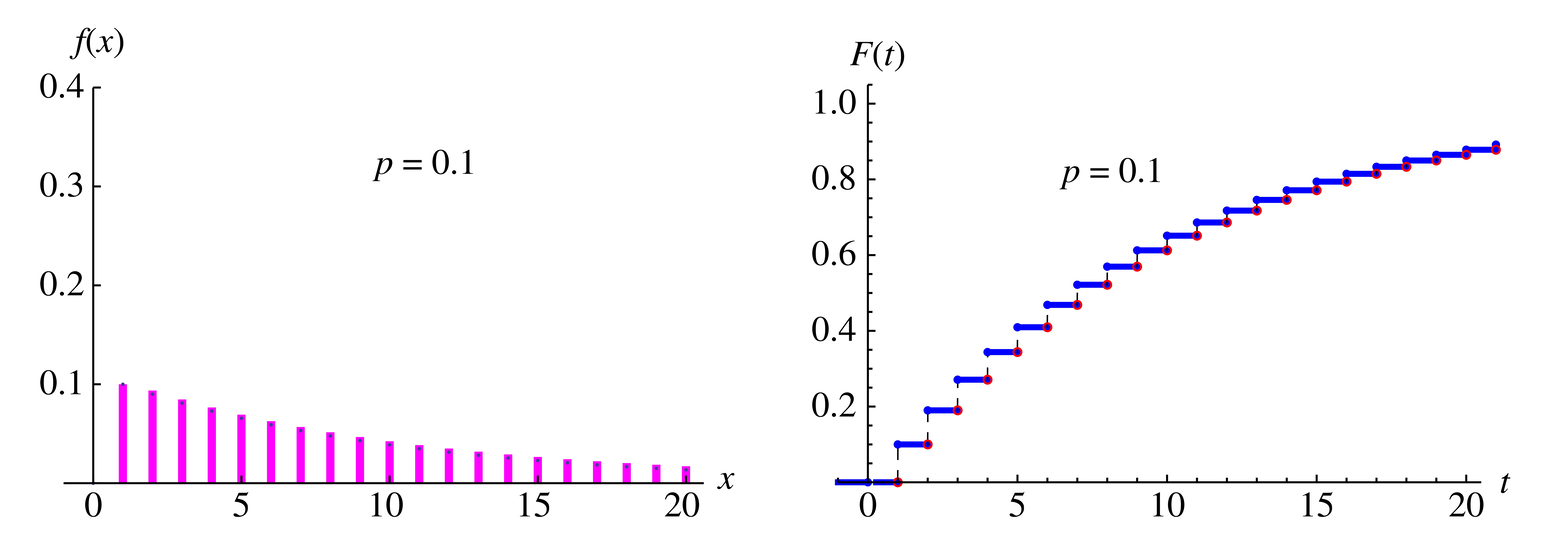
\includegraphics[width=.95\linewidth]{geom.png}
\caption{Geométrica}
\end{subfigure}\begin{subfigure}{.5\textwidth}\centering
\includegraphics[width=.95\linewidth]{binominal.png}
\caption{Binominal}
\end{subfigure}

\begin{subfigure}{.5\textwidth}\centering
\includegraphics[width=.95\linewidth]{negativabinominal.png}
\caption{Negativa binominal}
\end{subfigure}\begin{subfigure}{.5\textwidth}\centering
\includegraphics[width=.95\linewidth]{hyperg.png}
\caption{Hipergeométrica}
\end{subfigure}

\begin{subfigure}{.5\textwidth}\centering
\includegraphics[width=.95\linewidth]{gama.png}
\caption{$\Gamma$}
\end{subfigure}\begin{subfigure}{.5\textwidth}\centering
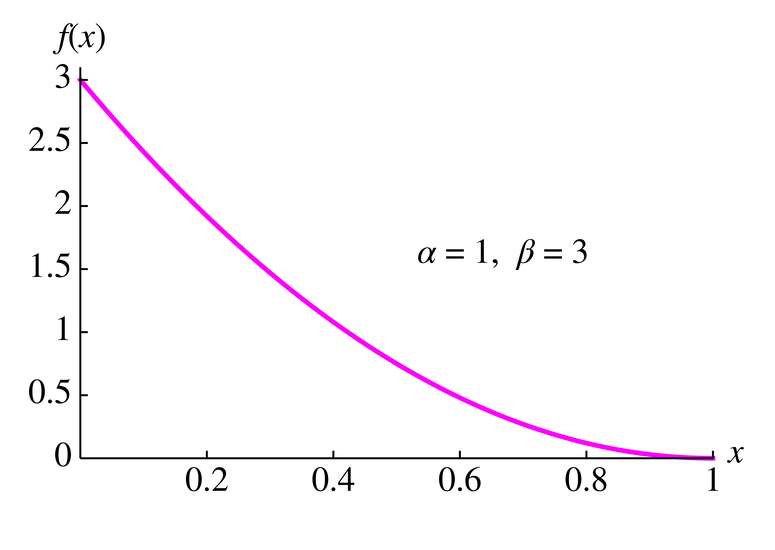
\includegraphics[width=.95\linewidth]{beta.png}
\caption{Beta}
\end{subfigure}

\begin{subfigure}{.5\textwidth}\centering
\includegraphics[width=.95\linewidth]{epsilon_lambda.png}
\caption{$\epsilon(\lambda)$}
\end{subfigure}\begin{subfigure}{.5\textwidth}\centering
\includegraphics[width=.95\linewidth]{normal.png}
\caption{Normal}
\end{subfigure}

\begin{subfigure}{.5\textwidth}\centering
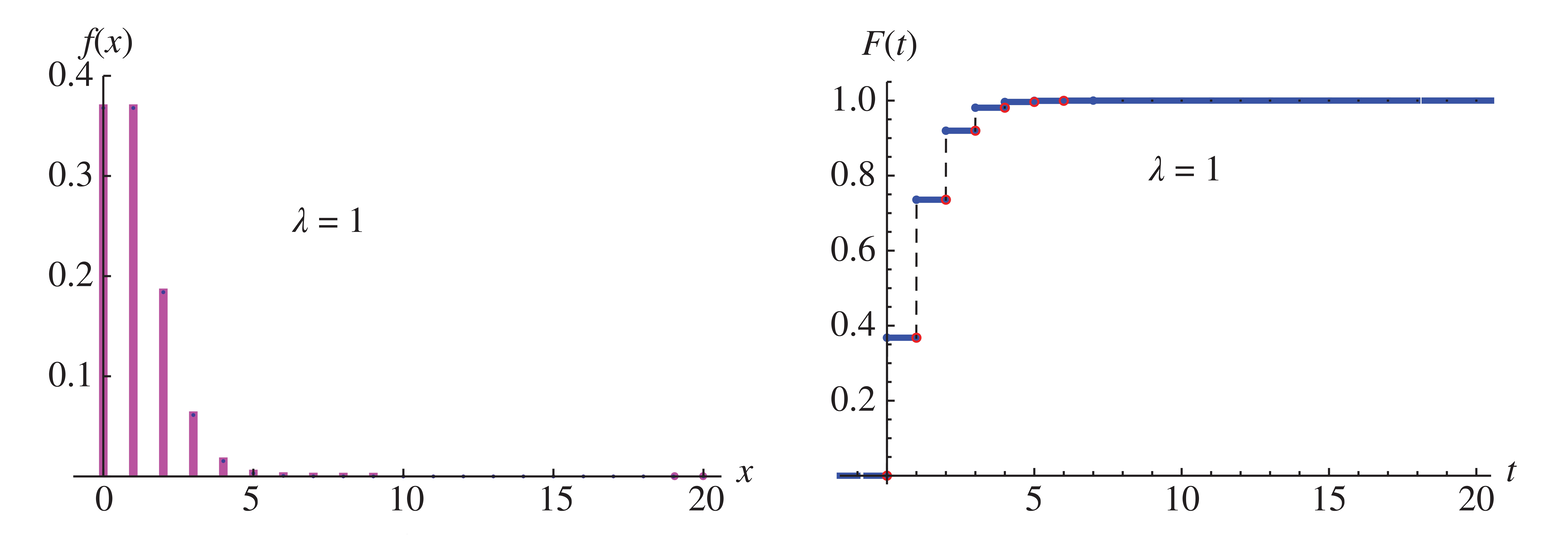
\includegraphics[width=.95\linewidth]{poisson.png}
\caption{Poisson}
\end{subfigure}\begin{subfigure}{.5\textwidth}\centering
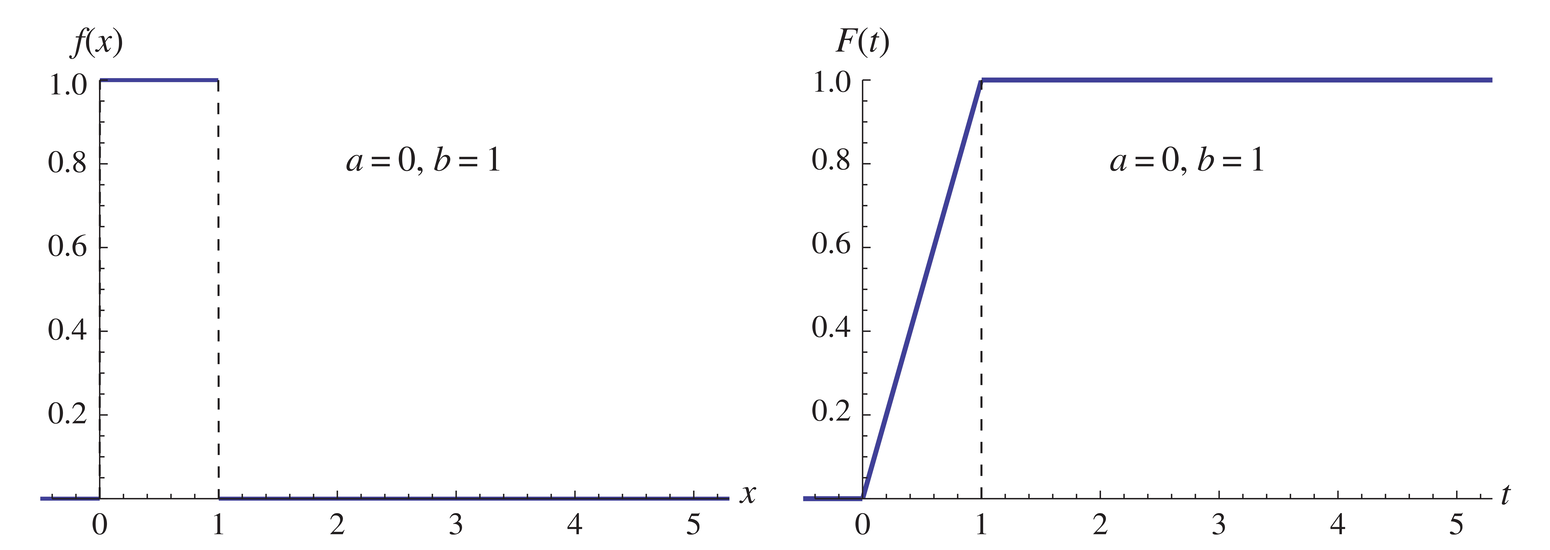
\includegraphics[width=.95\linewidth]{uniforme.png}
\caption{Uniforme}
\end{subfigure}
\end{figure}